


\subsection{Grid Options}
	
\begin{pgfplotsxykeylist}{\x minorgrids=\mchoice{true,false} (initially false),\x majorgrids=\mchoice{true,false} (initially false),grid=\mchoice{minor,major,both,none} (initially false)}
Enables/disables different grid lines. Major grid lines are placed at the normal tick positions (see |xmajorticks|) while minor grid lines are placed at minor ticks (see |xminorticks|). 

This example employs the coordinates defined on page~\pageref{page:plotcoords:src}.
\begin{codeexample}[]
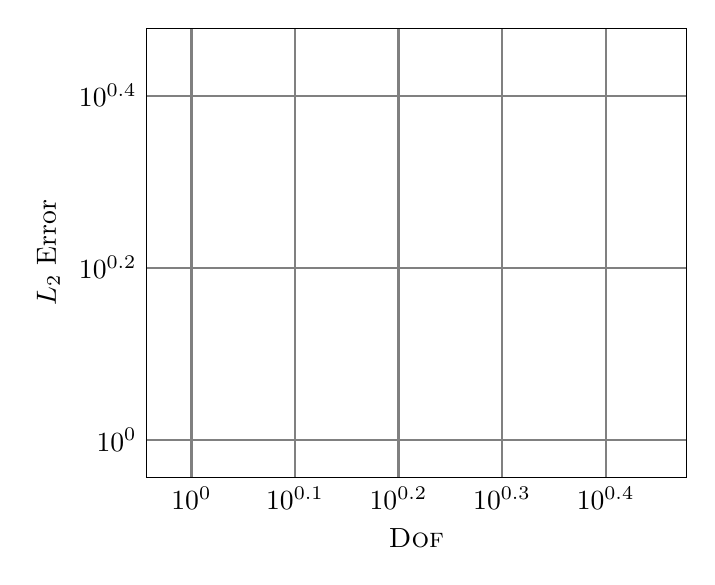
\begin{tikzpicture}
\begin{loglogaxis}[
	xlabel={\textsc{Dof}},
	ylabel={$L_2$ Error},
	grid=major
]
% see above for this macro:
\plotcoords
\end{loglogaxis}
\end{tikzpicture}
\end{codeexample}

\begin{codeexample}[]
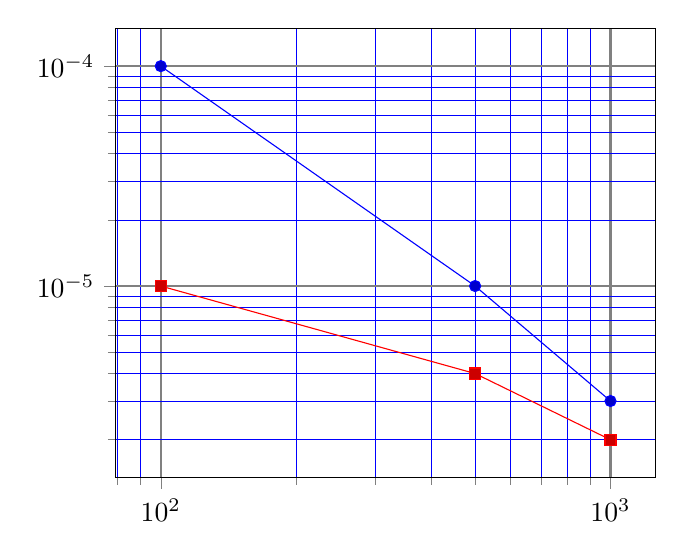
\begin{tikzpicture}
\begin{loglogaxis}[
	grid=both,
	tick align=outside,
	tickpos=left]
\addplot coordinates 
	{(100,1e-4) (500,1e-5) (1000,3e-6)};
\addplot coordinates 
	{(100,1e-5) (500,4e-6) (1000,2e-6)};
\end{loglogaxis}
\end{tikzpicture}
\end{codeexample}

Grid lines will be drawn before tick lines are processed, so ticks will be drawn on top of grid lines. You can configure the appearance of grid lines with the styles
\begin{codeexample}[code only]
\pgfplotsset{grid style={help lines}} % modifies the style `every axis grid'
\pgfplotsset{minor grid style={color=blue}} % modifies the style `every minor grid'
\pgfplotsset{major grid style={thick}} %modifies the style `every major grid'
\end{codeexample}
\end{pgfplotsxykeylist}


\subsection{Custom Annotations}
Often, one may want to add custom drawing elements or descriptive texts to an axis. These graphical elements should be associated to some logical coordinate, grid point, or perhaps just somewhere into the axis.

\PGFPlots\ assists with the following ways for how to add annotations:
\begin{enumerate}
	\item You can explicitly provide any \Tikz\ instruction like |\draw ... ;| into the axis. Here, the |axis cs| allows
	to provide coordinates of \PGFPlots.

	Furthermore, |rel axis cs| allows to position \Tikz\ elements relatively (like ``$50\%$ of the width).
	\item \PGFPlots\ can automatically generate nodes at every coordinate using its |nodes near coords| feature.
	\item \PGFPlots\ can automatically generate \Tikz\ labels for every coordinate (FIXME).
	\item \PGFPlots\ allows you to place nodes on a plot, using the |\addplot ... node[pos=|\meta{fraction}|] {};| feature.
\end{enumerate}
This section explains all of the approaches, except for the |nodes near coords| feature which is documented in its own section.

\subsubsection{Accessing Axis Coordinates in Graphical Elements}
\label{sec:axis:coords}%
\begin{coordinatesystem}{axis cs}
\PGFPlots\ provides a new coordinate system for use inside of an axis, the ``axis coordinate system'', |axis cs|.

It can be used to draw any \Tikz-graphics at axis coordinates. It is used like
\begin{codeexample}[code only]
\draw 
   (axis cs:18943,2.873391e-05) 
|- (axis cs:47103,8.437499e-06);
\end{codeexample}
\begin{codeexample}[]
\tikzstyle{every pin}=[fill=white,
	draw=black,
	font=\footnotesize]
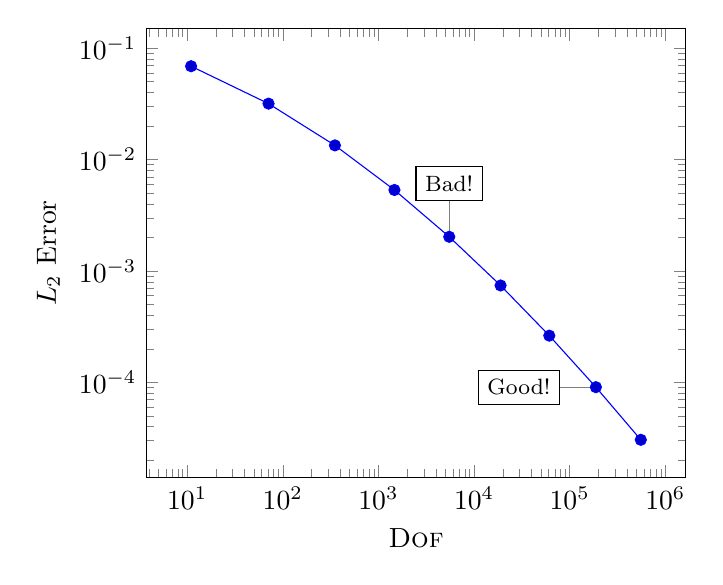
\begin{tikzpicture}
	\begin{loglogaxis}[
		xlabel={\textsc{Dof}},
		ylabel={$L_2$ Error}]

	\addplot coordinates {
		(11,     6.887e-02)
		(71,     3.177e-02)
		(351,    1.341e-02)
		(1471,   5.334e-03)
		(5503,   2.027e-03)
		(18943,  7.415e-04)
		(61183,  2.628e-04)
		(187903, 9.063e-05)
		(553983, 3.053e-05)
	};

	\node[coordinate,pin=above:{Bad!}] 
		at (axis cs:5503,2.027e-03) {};
	\node[coordinate,pin=left:{Good!}] 
		at (axis cs:187903,9.063e-05)	{};
	\end{loglogaxis}
\end{tikzpicture}
\end{codeexample}

\begin{codeexample}[]
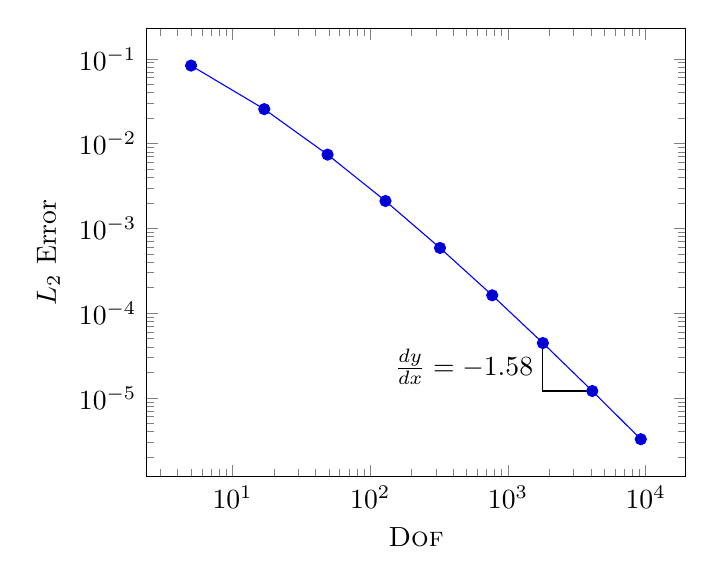
\begin{tikzpicture}
\begin{loglogaxis}[
	xlabel=\textsc{Dof},
	ylabel=$L_2$ Error
]
\draw 
		(axis cs:1793,4.442e-05)
	|-  (axis cs:4097,1.207e-05)
	node[near start,left] 
	{$\frac{dy}{dx} = -1.58$};

\addplot coordinates {
	(5,    8.312e-02)
	(17,   2.547e-02)
	(49,   7.407e-03)
	(129,  2.102e-03)
	(321,  5.874e-04)
	(769,  1.623e-04)
	(1793, 4.442e-05)
	(4097, 1.207e-05)
	(9217, 3.261e-06)
};
\end{loglogaxis}
\end{tikzpicture}
\end{codeexample}

\paragraph{Attention:} Whenever you draw additional graphics, consider using |axis cs|! It applies any logarithms, data scaling transformations or whatever \PGFPlots\ usually does!

There is also a low--level interface to access the transformations and coordinates, see Section~\ref{sec:pgfplots:lowlevel} on page~\pageref{sec:pgfplots:lowlevel}.
\end{coordinatesystem}

\begin{coordinatesystem}{rel axis cs}
The ``relative axis coordinate system'', |rel axis cs|, uses the complete axis vectors as units. That means `$x=0$' denotes the point on the lower $x$ axis range and `$x=1$' the point on the upper $x$ axis range (see the remark below for |x dir=reverse|).

\pgfplotsexpensiveexample
\begin{codeexample}[]
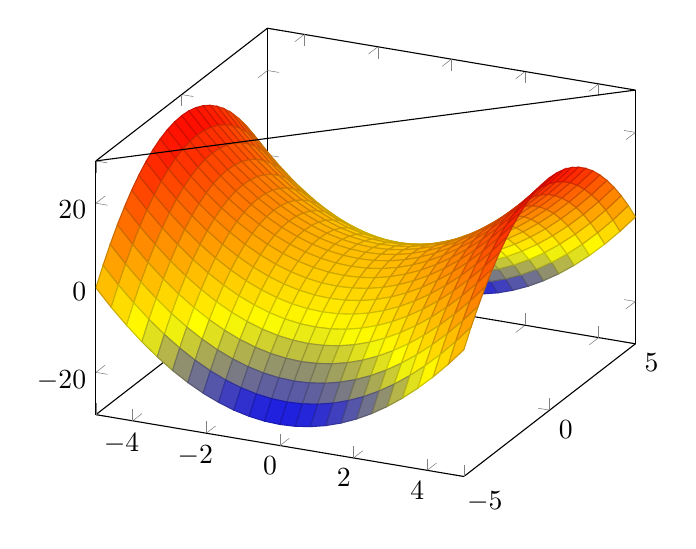
\begin{tikzpicture}
\begin{axis}

	\addplot3[surf] {x^2 - y^2};
	\draw  (rel axis cs:0,0,1) 
		-- (rel axis cs:1,1,1);
\end{axis}
\end{tikzpicture}
\end{codeexample}

\pgfplotsexpensiveexample
\begin{codeexample}[]
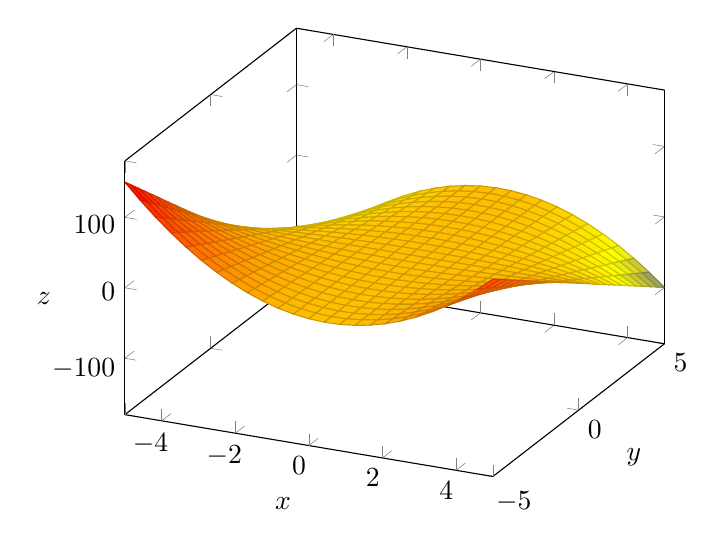
\begin{tikzpicture}
\begin{axis}[
	xlabel=$x$,
	ylabel=$y$,
	zlabel=$z$,
	every axis x label/.style={
		at={(rel axis cs:0.5,-0.15,-0.15)}},
	every axis y label/.style={
		at={(rel axis cs:1.15,0.5,-0.15)}},
	every axis z label/.style={
		at={(rel axis cs:-0.15,-0.15,0.5)}},
]

	\addplot3[surf] {x*(1-x)*y};
\end{axis}
\end{tikzpicture}
\end{codeexample}

	Points identified by |rel axis cs| use the syntax

		|(rel axis cs:|\meta{x}|,|\meta{y}|)| or

		|(rel axis cs:|\meta{x}|,|\meta{y}|,|\meta{z}|)| 
	
	\noindent where \meta{x}, \meta{y} and \meta{z} are coordinates or constant mathematical expressions. The second syntax is only available in three dimensional axes.

	There is one specialty: if you reverse an axis (with |x dir=reverse|), points provided by |rel axis cs| will be \emph{unaffected} by the axis reversal. This is intended to provide consistent placement even for reversed axes. Use |allow reversal of rel axis cs=false| to disable this feature.

There is also a low--level interface to access the transformations and coordinates, see Section~\ref{sec:pgfplots:lowlevel} on page~\pageref{sec:pgfplots:lowlevel}.
\end{coordinatesystem}

\begin{predefinednode}{current plot begin}
	This coordinate will be defined for every plot and can be used is \meta{trailing path commands} or after a plot. It is the first coordinate of the current plot.	
\end{predefinednode}

\begin{predefinednode}{current plot end}
	This coordinate will be defined for every plot. It is the last coordinate of the current plot.	
\end{predefinednode}

\begin{pgfplotskey}{allow reversal of rel axis cs=\mchoice{true,false} (initially true)}
	A fine-tuning key which specifies how to deal with |x dir=reverse| and |rel axis cs| and |ticklabel cs|.

	The initial configuration |true| means that points placed with |rel axis cs| and/or |ticklabel cs| will be at the same position inside of the axes even if its ordering has been reversed. The choice |false| will disable the special treatment of |x dir=reverse|.
\end{pgfplotskey}

\subsubsection{Placing Nodes on Coordinates of a Plot}
{
\tikzset{external/figure name/.add={}{nodes_}}%
The |\addplot| command is not only used for \PGFPlots, it can also carry additional drawing instructions which are handed over to \Tikz\ after the plot's path is complete. Among others, this can be used to add further nodes on the path.

\begin{key}{/tikz/pos=\marg{fraction}}
	The \meta{fraction} identifies a part of the recently completed plot if it is used before the trailing semicolon:
\pgfplotsexpensiveexample
\begin{codeexample}[]
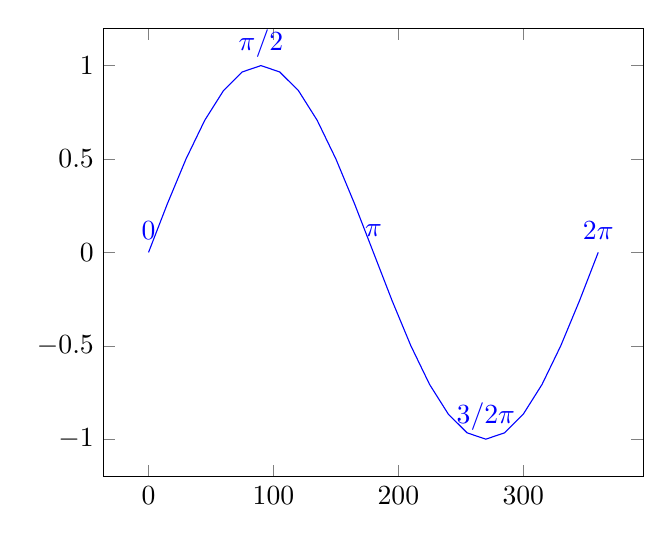
\begin{tikzpicture}
	\begin{axis}
	\addplot[blue,domain=0:360] {sin(x)} 
	[yshift=8pt]
		node[pos=0] {$0$} 
		node[pos=0.25] {$\pi/2$}
		node[pos=0.5] {$\pi$}
		node[pos=0.75] {$3/2\pi$}
		node[pos=1] {$2\pi$}
	;
	\end{axis}
\end{tikzpicture}
\end{codeexample}
\noindent Here, the |[yshift=8pt]| tells \Tikz\ to shift all following nodes upwards. The |node[pos=0] {$0$}| instruction tells \Tikz\ to add a text node at $0\%$ of the recently completed plot. The relative position $0\%$ (|pos=0|) refers to the first coordinate which has been seen by \PGFPlots, and $100\%$ (|pos=1|) refers to the last coordinate. Any value between $0$ and $1$ is interpolated inbetween. Note that all these nodes belong to the plot's visualization (which is terminated by the semicolon). Consequently, all these nodes inherit the same graphic settings (like color choices).

	The position on the plot is computed by \PGFPlots\ using \emph{logical} coordinates. In other words: it computes the overal length of the curve before the curve is projected to screen coordinates and identifies the desired position\footnote{This can be a time-consuming process. Consider using the external library if you have lots of such figures.}. Afterwards, it projects the final position to screen coordinates. Thus, the |pos|ition identifies a position on the plot which is always the same, even in case of a rotated three-dimensional axis. \PGFPlots\ will linearly interpolate the fraction between successive coordinates.

	Valid choices for \meta{fraction} are any numbers in the range $[0,1]$.

	Note that |pos| may not be available (or even useful) for all plot handlers. The \PGFPlots\ team may choose to add plot-type specific implementations in the future.
\end{key}

\begin{key}{/tikz/sloped (initially false)}
	Providing the \Tikz\ key |sloped| to a node identified by |pos| causes it to be rotated such that it adapts to the plot's gradient.
\pgfplotsexpensiveexample
\begin{codeexample}[]
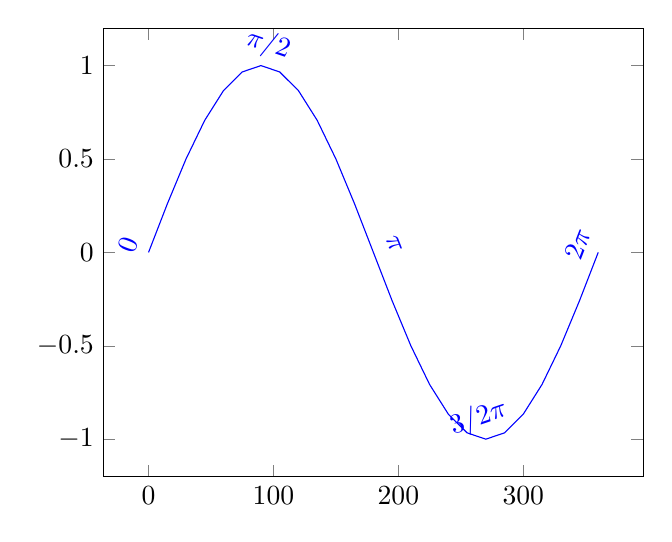
\begin{tikzpicture}
	\begin{axis}
	\addplot[blue,domain=0:360] {sin(x)} 
	[every node/.style={yshift=8pt},sloped]
		node[pos=0] {$0$} 
		node[pos=0.25] {$\pi/2$}
		node[pos=0.5] {$\pi$}
		node[pos=0.75] {$3/2\pi$}
		node[pos=1] {$2\pi$}
	;
	\end{axis}
\end{tikzpicture}
\end{codeexample}
	Note that the sequence in which |sloped| and shift transformations are applied is important: if shifts are applied first (as would be the case without the |every node/.style| construction), the shifts do not respect the rotation. If |sloped| is applied first, any subsequent shifts will be applied in the \emph{rotated} coordinates. Thus, the case |every node/.style={yshift=8pt}| shifts every node by |8pt| in direction of its normal vector.
\end{key}

\begin{key}{/tikz/allow upside down=\mchoice{true,false} (initially false)}
	If |/tikz/sloped| is enabled and one has some difficult line plot, the transformation may cause nodes to be drawn upside down. The default configuration |allow upside down=false| will switch the rotation matrix, whereas |allow upside down| allows this case.
\end{key}

\begin{key}{/tikz/pos segment=\marg{segment index} (initially empty)}
	Occasionally, one has a single plot which consists of multiple segments (like those generated by |empty line=jump| or |contour prepared|). The individual segments will typically have different lengths, so it is tedious to identify a position on one of these segments.

	If |pos segment=|\meta{segment index} is provided, the key |pos=|\meta{fraction} is interpreted relative to the provided segment rather than the whole plot. The argument \meta{segment index} is an integer, where $0$ denotes the first segment.
\begin{codeexample}[]
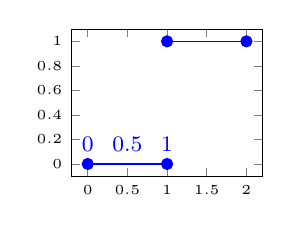
\begin{tikzpicture}
\begin{axis}[tiny]
\addplot coordinates {
	(0,0) (1,0) 

	(1,1) (2,1)
}
	[pos segment=0,yshift=7pt,font=\footnotesize]
	node[pos=0] {0} node[pos=0.5] {0.5} node[pos=1] {1};
\end{axis}
\end{tikzpicture}
\end{codeexample}
	Here, the plot has two segments. However, all three annotation nodes are placed with |pos segment=0|.

\pgfplotsexpensiveexample
\begin{codeexample}[]
\begin{tikzpicture}
\begin{axis}
\addplot3[contour gnuplot,domain=0:1] {x*y}
	[sloped,
	 allow upside down,
	 pos segment=2,
	 every node/.style={yshift=7pt}]
	node[pos=0] {0} node[pos=0.5] {0.5} node[pos=1] {1}
	;

\end{axis}
\end{tikzpicture}
\end{codeexample}
	This plot has four segments (which are generated automatically by the plot handler). The annotation nodes are placed
	on the third segment, where |sloped| causes them to be rotated, |allow upside down| improves the rendering of the `$0$', and |every node/.style| install a shift in direction of the normal vector (see the documentation of |sloped| for details).
\end{key}


}

